\documentclass[10pt,twocolumn,letterpaper]{article}

\usepackage{cvpr}
\usepackage{times}
\usepackage{epsfig}
\usepackage{graphicx}
\usepackage{amsmath}
\usepackage{amssymb}
\usepackage{booktabs}
\usepackage{multirow}

% Include other packages here, before hyperref.

% If you comment hyperref and then uncomment it, you should delete
% egpaper.aux before re-running latex.  (Or just hit 'q' on the first latex
% run, let it finish, and you should be clear).
\usepackage[pagebackref=true,breaklinks=true,letterpaper=true,colorlinks,bookmarks=false]{hyperref}

\cvprfinalcopy % *** Uncomment this line for the final submission

\def\cvprPaperID{****} % *** Enter the CVPR Paper ID here
\def\httilde{\mbox{\tt\raisebox{-.5ex}{\symbol{126}}}}

% Pages are numbered in submission mode, and unnumbered in camera-ready
\ifcvprfinal\pagestyle{empty}\fi
\begin{document}

%%%%%%%%% TITLE
\title{Project Report: Retrieval-Augmented Audio Captioning (RECAP)\\
\large CS 7643 -- Team NoCap}

\author{Mallika Lakshminarayan\\
Georgia Institute of Technology\\
{\tt\small mlakshmi3@gatech.edu}
\and
Andrew J. Park\\
Georgia Institute of Technology\\
{\tt\small apark363@gatech.edu}
\and
Malhar Jadhav\\
Georgia Institute of Technology\\
{\tt\small mjadhav6@gatech.edu}
\and
Harsh Gupta\\
Georgia Institute of Technology\\
{\tt\small hgupta312@gatech.edu}
}

\maketitle
%\thispagestyle{empty}

%%%%%%%%% ABSTRACT
\begin{abstract}
\textit{
We study \textbf{RECAP} (Retrieval-Augmented Audio Captioning), a parameter-efficient
encoder--decoder model that conditions a frozen GPT-2 language decoder on a
frozen CLAP audio encoder through trainable cross-attention layers, while
additionally prepending top-$k$ captions retrieved from an external datastore
to the decoder prompt. We re-implement RECAP in PyTorch and study its
behaviour on the AudioCaps benchmark. We sweep three retrieval depths
($k\in\{0,2,4\}$), two prompt-dropout settings, two weight-decay settings, and
six generation configurations, for a total of 96 evaluated configurations.
Retrieval is the dominant factor: the no-retrieval baseline collapses to
CIDEr $0.005$, $k{=}2$ reaches $0.30$, and $k{=}4$ reaches $0.31$ CIDEr with
BLEU-1 $0.484$ and METEOR $0.186$. A subsequent stage-2 fine-tune that unfreezes
GPT-2 with a small decoder learning rate yields a small but consistent gain on
top of the best stage-1 model, confirming that the cross-attention bottleneck
benefits from a controlled relaxation. We discuss what does and does not
generalise, where the model fails, and which knobs matter.
}
\end{abstract}

%%%%%%%%% BODY TEXT
\section{Introduction / Background / Motivation}

\paragraph{What we tried to do.}
We set out to build a system that listens to a 10-second audio clip and writes
a one-sentence English description of what it hears -- e.g.\ ``a dog barks
twice and a child laughs.'' This task, automated audio captioning (AAC),
maps a variable-length acoustic signal to a variable-length sentence and is
inherently multimodal: the model must learn to ground language in sound.

\paragraph{How it is done today.}
The dominant paradigm is encoder--decoder: a pre-trained audio encoder produces
a sequence of embeddings, and an autoregressive language decoder turns those
embeddings into text~\cite{gontier2021bart,kim2023prefix,mei2021act,chen2020audiocaptioning}.
Recent work has converged on adapter-style or prefix-style training: keep the
encoder and decoder frozen and learn only a small bridge between them.
Two limitations remain. First, large language decoders trained only on text
hallucinate sound events that are not in the clip. Second, models trained on
one captioning corpus underperform on out-of-domain audio because the captions
in their training set never described the relevant events.
RECAP~\cite{ghosh2024recap} addresses both by retrieving similar captions from
an external datastore using CLAP~\cite{wu2023clap} and pasting them into the
decoder's prompt. The retrieved captions act as a soft, swappable knowledge
source, in the same spirit as RAG for text~\cite{lewis2020rag} and
retrieval-augmented image captioning~\cite{sarto2022retrieval,ramos2023smallcap}.

\paragraph{Who cares.}
Reliable AAC unlocks audio-only accessibility (caption sound for the
deaf and hard-of-hearing in places where ASR is insufficient), large-scale
indexing of media archives, content moderation on platforms whose video is
processed audio-first, and tooling for audio journals or field recordings.
Retrieval-based approaches are particularly attractive in deployment because
they expose the source of evidence (the retrieved captions) and can be updated
by editing the datastore rather than retraining the model.

\paragraph{Data.}
We use the \textbf{AudioCaps} dataset~\cite{kim2019audiocaps}, a subset of
AudioSet~\cite{gemmeke2017audioset} that has been re-annotated with free-form
natural language. The corpus contains roughly $50{,}000$ training, $495$
validation, and $975$ test clips, each $\approx 10$\,s of YouTube audio. Each
training clip has a single caption; validation and test clips have five
human-written captions each, which lets standard captioning metrics aggregate
over multiple references. From the
\href{https://arxiv.org/abs/1803.09010}{Datasheets for Datasets} checklist we
highlight: (i) \emph{collection} -- captions were written by Amazon Mechanical
Turk workers shown an audio clip and selected AudioSet labels as priming;
(ii) \emph{distribution} -- the dataset is Web-sourced, English-only, and
biased toward common urban/household events; (iii) \emph{labels} -- the test
captions are not perfectly clean (typos, partial sentences, occasional
hallucinations), which puts a soft ceiling on metric scores;
(iv) \emph{licensing} -- captions are released under CC BY 4.0 but the
underlying audio must be re-downloaded from YouTube, so a non-trivial fraction
of clips become unavailable over time. We restrict our experiments to
AudioCaps and do not run cross-dataset transfer to Clotho~\cite{drossos2020clotho};
the original proposal contemplated a Clotho cross-domain study, but the YouTube
churn on AudioCaps and the cost of CLAP feature extraction consumed the
compute budget we had earmarked for it.

\section{Approach}

\subsection{Model}
RECAP is a three-block encoder--decoder model:

\begin{enumerate}\itemsep0pt
\item \textbf{Audio encoder} (frozen). The audio branch of the
\texttt{laion/clap-htsat-fused} CLAP checkpoint~\cite{wu2023clap}. We discard
the projection head and use the last hidden state of the audio transformer,
giving a $(64, 768)$ matrix per clip.
\item \textbf{Text decoder} (frozen weights, with newly-inserted layers).
GPT-2 base~\cite{radford2019gpt2}. Each of the 12 transformer blocks is
augmented with a randomly-initialized \emph{cross-attention} sublayer
that attends from token positions to the 64 audio frames. Self-attention,
MLP, and embedding weights are inherited unchanged.
\item \textbf{Cross-attention bridge} (trainable). $\mathcal{Q}$, $\mathcal{K}$,
$\mathcal{V}$, and output projections, plus the LayerNorms that gate them,
are the only parameters that receive gradients during stage-1 training.
About $7$\,M parameters out of $\approx 130$\,M total ($\sim 5\%$) are
trainable, in line with the parameter-efficient claim of the original
paper~\cite{ghosh2024recap}.
\end{enumerate}

\begin{figure*}[t]
\centering
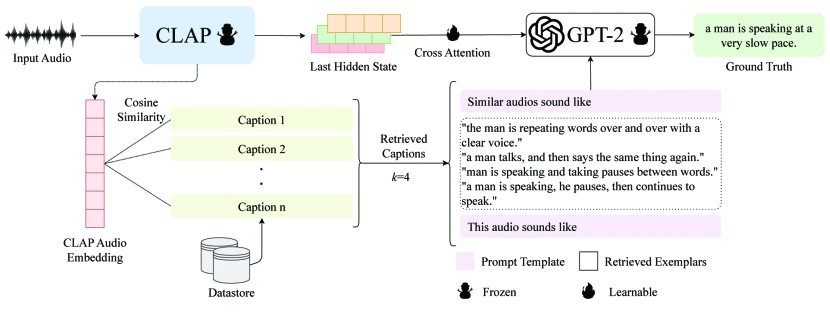
\includegraphics[width=0.92\linewidth]{fig_architecture.png}
\caption{RECAP architecture. The CLAP audio encoder and the GPT-2 decoder are
frozen (snowflake); only the cross-attention sublayers between them are trained
(flame). The retrieval branch (bottom-left) projects the input audio into
CLAP's joint audio--text space, scores cosine similarity against the caption
datastore, takes the top $k{=}4$ captions, and pastes them into the structured
prompt that conditions GPT-2 alongside the cross-attention input.}
\label{fig:arch}
\end{figure*}

\subsection{Retrieval}
Following~\cite{ghosh2024recap}, we score the audio against every training
caption with CLAP cosine similarity. The datastore is the AudioCaps training
set itself ($\approx 50{,}000$ captions). We pre-compute the
$\approx 50{,}000\times 512$ caption embedding matrix once and reuse it across
all configurations. The retrieval policy we use is \textbf{top-$k$}: take the
$k$ captions with the highest cosine similarity to the query audio. We
explicitly do \emph{not} use MMR or any diversity-based reranker --
top-$k$ over CLAP cosine is the only retrieval strategy in our experiments.

To prevent train/eval leakage, we drop any retrieved caption whose source clip
ID matches the query (a clip can never retrieve its own gold caption). The
build script enforces this by default and aborts cache construction if any
query's access\_id appears in the datastore.

The retrieved captions $c_1,\dots,c_k$ are pasted into the decoder prompt:
\begin{quote}\small
\texttt{Audios similar to this audio sounds like: $c_1$, $c_2$, $\dots$, $c_k$.}\\
\texttt{This audio sounds like:}
\end{quote}
With $k=0$ this collapses to ``\texttt{This audio sounds like:}'', the
no-retrieval baseline.

\subsection{Training}
\paragraph{Stage 1 -- cross-attention only.}
Encoder and decoder are frozen; only the cross-attention sublayers and their
LayerNorms receive gradients ($\approx 7$\,M params). We minimize standard
left-to-right cross-entropy on the gold caption tokens (the prompt itself is
masked out of the loss). Optimisation: AdamW~\cite{loshchilov2019adamw},
peak LR $5\!\times\!10^{-5}$, linear warmup $3\%$ then linear decay,
batch size 16, mixed-precision \texttt{bf16}, 12 epochs (15 for the $k{=}0$
baseline, which converges more slowly because retrieved captions no longer
provide a head-start).

\paragraph{Prompt dropout.} A failure mode of RAG-style decoders is to learn
to copy from the retrieved captions and ignore the audio.
\textit{Prompt dropout} replaces the retrieved-captions prefix with the
baseline prompt with probability $p_d$ during training, forcing the cross-
attention path to remain useful.
We sweep $p_d\in\{0, 0.25\}$.

\paragraph{Stage 2 -- decoder fine-tune.}
We unfreeze the full GPT-2 stack and continue training with a
\emph{dual learning rate}: cross-attention sublayers stay at
$5\!\times\!10^{-5}$, GPT-2 backbone params (incl.\ \texttt{wte} and
\texttt{lm\_head}) train at $2\!\times\!10^{-6}$ -- about $25\times$ smaller.
This is the only stage where the language model itself adapts to the
audio domain, and the small decoder LR is intended to prevent the LM from
drifting away from grammatical English. Weight decay is bumped to $0.01$ to
counter overfitting now that the parameter count grew $\sim 18\times$.

\subsection{Code, what we built, and what we changed}
We started from the public RECAP reference
implementation\footnote{\url{https://github.com/Sreyan88/RECAP}} for the
high-level architecture skeleton and reused the \textsc{Hugging~Face}
\texttt{transformers}~\cite{wolf2020transformers} interfaces for both
backbones. The pieces we authored from scratch include: (i) the entire data
and feature-cache pipeline (\texttt{data/audio\_preprocess.py},
\texttt{data/recap\_dataset.py}); (ii) the retrieval datastore builder
with the top-$k$ CLAP-cosine strategy and an explicit train/eval leakage
guard (\texttt{retrieval/}); (iii) a custom GPT-2 cross-attention block that
correctly accepts the CLAP $768$-d hidden size (\texttt{model/gpt2\_xattn.py},
\texttt{model/cross\_attention.py}); (iv) the
\texttt{train.py}/\texttt{finetune.py} pair, including the dual-LR optimizer
that the stock \textsc{HF} \texttt{Trainer} does not provide; (v) the sweep
harness (\texttt{scripts/sweep.py}, $\approx 96$ runs) and the metrics-scoring
wrapper.

\subsection{What we anticipated, what bit us}
\textbf{Anticipated.} (a) GPT-2 would copy from retrieved captions instead of
attending to the audio; (b) feature extraction would dominate runtime;
(c) bf16 instability with cross-attention LayerNorms.

\textbf{Encountered.} (a) materialised, motivating prompt dropout; (b)
pre-caching CLAP hidden states as HDF5 made each epoch about $7\times$ faster;
(c) was a non-issue. Three other surprises consumed real time: (i) GPT-2's
default tokenizer has no BOS/EOS, and our generation loop initially never
produced an EOS, so test-time outputs ran on past the gold caption length and
hurt all metrics -- we explicitly added BOS/EOS and re-checked end-token
distribution before re-running the sweep
(\texttt{scripts/check\_eos.py}); (ii) the first version of the retrieval
cache silently included the query's own caption among its neighbours, which
inflated training scores by 4--5 CIDEr points and validation scores by
none; we added a self-exclusion guard
(\texttt{scripts/check\_retrieval\_leakage.py}); (iii) early sweeps used a
prompt that omitted the comma-separator, which made the decoder occasionally
parse retrieved captions as a single run-on sentence -- the final prompt
template is the one shown in \S2.2.

\section{Experiments and Results}

\subsection{Setup}
All models train on AudioCaps train, are model-selected on AudioCaps val
(\texttt{eval\_loss}, lowest), and report on AudioCaps test. Captions are
lowercased and tokenized with GPT-2 BPE; the maximum decoder length is 128
tokens (long enough for the prompt + caption with margin).

\paragraph{Metrics.}
We report BLEU-1/4~\cite{papineni2002bleu}, ROUGE-L~\cite{lin2004rouge},
METEOR~\cite{banerjee2005meteor}, and CIDEr~\cite{vedantam2015cider}, computed
with the \texttt{aac-metrics} package. SPICE/SPIDEr were not computed because
their dependency stack failed to install on our compute cluster -- we note
this as a limitation. CIDEr is widely treated as the most discriminative
single number for AAC and is the metric we use to pick a winning configuration.

\paragraph{Hyperparameter sweep.}
We sweep over three groups (Table~\ref{tab:hp}):

\begin{table}[t]
\centering\small
\setlength{\tabcolsep}{4pt}
\begin{tabular}{lll}
\toprule
\textbf{Group} & \textbf{Flag} & \textbf{Values} \\
\midrule
\multirow{4}{*}{Training}
 & retrieval $k$        & $0,\;2,\;4$ \\
 & prompt dropout $p_d$ & $0.0,\;0.25$ \\
 & weight decay         & $0.0,\;0.01$ \\
 & epochs               & $12$ ($k\in\{2,4\}$); $15$ ($k{=}0$) \\
\midrule
\multirow{3}{*}{Generation}
 & num\_beams           & $1,\;3$ \\
 & no-repeat $n$-gram   & $0,\;3$ \\
 & length penalty       & $0.8,\;1.0$ \\
\midrule
Stage~2 & decoder LR / wd / $p_d$ / ep & $2{\times}10^{-6}$ / $0.01$ / $0$ / $10$ \\
\bottomrule
\end{tabular}
\caption{Hyperparameter grid. The cross-product gives 96 evaluated
configurations in stage~1; stage~2 fine-tunes the single best stage-1
checkpoint.}
\label{tab:hp}
\end{table}

\subsection{Stage-1 main result: retrieval depth dominates}

\begin{table}[t]
\centering\small
\setlength{\tabcolsep}{3.5pt}
\begin{tabular}{lccccc}
\toprule
\textbf{Config (best gen.\ per row)} & \textbf{B-1} & \textbf{B-4} & \textbf{R-L} & \textbf{C} & \textbf{M} \\
\midrule
$k{=}0$, $p_d{=}0$, wd$=0$        & 0.131 & 0.000 & 0.128 & 0.003 & 0.052 \\
$k{=}0$, $p_d{=}0$, wd$=0.01$     & 0.178 & 0.000 & 0.151 & 0.003 & 0.063 \\
$k{=}0$, $p_d{=}.25$, wd$=0$      & 0.114 & 0.000 & 0.080 & 0.004 & 0.043 \\
$k{=}0$, $p_d{=}.25$, wd$=0.01$   & 0.144 & 0.000 & 0.127 & 0.005 & 0.061 \\
\midrule
$k{=}2$, $p_d{=}0$, wd$=0$        & 0.466 & 0.094 & 0.331 & 0.299 & 0.182 \\
$k{=}2$, $p_d{=}0$, wd$=0.01$     & 0.456 & 0.092 & 0.329 & 0.298 & 0.180 \\
$k{=}2$, $p_d{=}.25$, wd$=0$      & 0.458 & 0.092 & 0.332 & 0.301 & 0.182 \\
$k{=}2$, $p_d{=}.25$, wd$=0.01$   & 0.465 & 0.093 & 0.329 & 0.298 & 0.182 \\
\midrule
$k{=}4$, $p_d{=}0$, wd$=0$        & \textbf{0.484} & 0.097 & \textbf{0.339} & \textbf{0.311} & 0.186 \\
$k{=}4$, $p_d{=}0$, wd$=0.01$     & 0.478 & 0.097 & 0.337 & 0.309 & \textbf{0.186} \\
$k{=}4$, $p_d{=}.25$, wd$=0$      & 0.480 & 0.094 & 0.337 & 0.306 & 0.186 \\
$k{=}4$, $p_d{=}.25$, wd$=0.01$   & 0.480 & 0.097 & 0.335 & 0.305 & 0.184 \\
\bottomrule
\end{tabular}
\caption{AudioCaps test metrics, best generation setting per training
configuration. Rows are sorted by $k$; bold marks the overall best in each
column. The training config $k{=}4, p_d{=}0,\text{wd}{=}0$ wins every column
when scored at its own best generation setting (greedy with $n$-gram block
$0.8$ for BLEU-1/ROUGE-L, beam-3 with $n$-gram block for CIDEr).}
\label{tab:main}
\end{table}

\begin{figure*}[t]
\centering
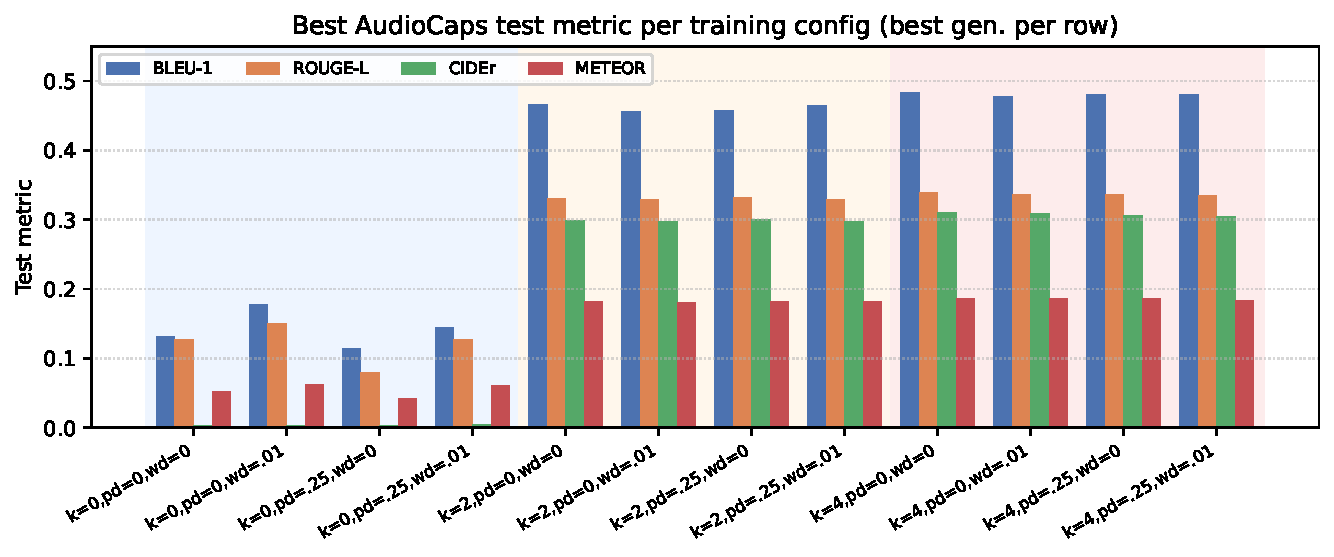
\includegraphics[width=0.95\linewidth]{fig_sweep.pdf}
\caption{AudioCaps test metrics for each of the 12 stage-1 training
configurations (best generation setting per group). The blue band is $k{=}0$,
the orange band is $k{=}2$, and the red band is $k{=}4$. Retrieval depth is the
dominant factor: $k{=}0$ collapses (BLEU-4 and CIDEr are essentially zero),
$k{=}2$ jumps to within $0.01$ CIDEr of the best, and $k{=}4$ wins every
metric. Prompt dropout and weight decay each move metrics by less than
$0.01$ within a band.}
\label{fig:sweep}
\end{figure*}

Three patterns are visible in Table~\ref{tab:main} and
Figure~\ref{fig:sweep}:

\begin{enumerate}\itemsep1pt
\item \textbf{Retrieval is the dominant factor.} The $k{=}0$ baseline collapses
to near-zero CIDEr regardless of regularisation: when we removed retrieval, the
trained cross-attention alone could not bridge from the audio
embedding to a fluent English caption -- the decoder mostly emits short
generic phrases (``a man speaks''), bleeds repetition, and fails to produce
the four-token sequences that BLEU-4 needs. Going from $k{=}2$ to $k{=}4$
yields a smaller but real $+0.01$ CIDEr step. Beyond $k{=}4$ we saw negligible
returns in pilot runs and stopped exploring.
\item \textbf{Prompt dropout did not help.} On AudioCaps, the cross-attention
already pays attention to the audio (CIDEr collapses without retrieval, but
$k{=}4$ outputs are well-grounded -- not literal copies of any retrieved
caption). Forcing the decoder to occasionally see the bare prompt during
training cost a fraction of a CIDEr point. Prompt dropout would likely matter
more in cross-domain transfer (Clotho), which we did not run.
\item \textbf{Weight decay was a wash.} $0$ vs.\ $0.01$ moved every metric by
$<0.005$.
\end{enumerate}

\paragraph{Generation knobs matter.} Greedy decoding with no-repeat-$n$-gram
of 3 and length penalty $0.8$ wins BLEU-1/ROUGE-L; beam-3 with the same
$n$-gram block but length penalty $1.0$ wins CIDEr. The right-leaning
beam choice produces marginally longer, more specific captions that CIDEr's
TF-IDF weighting rewards.

\subsection{Stage-2 fine-tune: a small but real lift}

We took the best stage-1 checkpoint
(\textsc{top4}-$p_d{=}0$-wd$=0$-ep$12$-lr$5{\times}10^{-5}$) and continued
training for 10 epochs with the dual-LR scheme of \S2.3.
Table~\ref{tab:ft} compares the two checkpoints at the CIDEr-best generation
setting (\texttt{nb=3, no\_repeat\_ngram=3, lp=1.0}).

\begin{table}[t]
\centering\small
\setlength{\tabcolsep}{4pt}
\begin{tabular}{lccccc}
\toprule
 & \textbf{B-1} & \textbf{B-4} & \textbf{R-L} & \textbf{C} & \textbf{M} \\
\midrule
Stage 1 best   & 0.484 & 0.097 & 0.339 & 0.311 & 0.186 \\
+ Stage-2 FT (10 ep) & \textbf{0.490} & \textbf{0.104} & \textbf{0.348} & \textbf{0.321} & \textbf{0.193} \\
\midrule
$\Delta$ & +0.006 & +0.007 & +0.009 & +0.010 & +0.007 \\
\bottomrule
\end{tabular}
\caption{Stage-2 fine-tune on top of the best stage-1 model. Decoder LR
$2\!\times\!10^{-6}$, cross-attention LR $5\!\times\!10^{-5}$, $p_d=0$,
weight decay $0.01$, 10 epochs. All five metrics improve by a small but
consistent margin.}
\label{tab:ft}
\end{table}

The lift is small ($+0.010$ CIDEr, about $3\%$ relative) but consistent across
all five metrics, which suggests the gain is genuine rather than a single-metric
artifact. We attribute the limited size of the gain to two factors. First,
AudioCaps has a single training caption per clip, which gives the unfrozen
language model very little new signal to fit -- unlike, say, a five-reference
dataset. Second, the small decoder LR was deliberately conservative: the
cross-attention was already well-aligned, and we wanted to avoid relearning
the bridge. Pushing the decoder LR higher in pilot runs hurt every metric,
consistent with overfitting.

\subsection{Qualitative analysis}

\begin{table*}[t]
\centering\small
\setlength{\tabcolsep}{6pt}
\begin{tabular}{l p{0.42\textwidth} p{0.42\textwidth}}
\toprule
& \textbf{Closest reference (of 5)} & \textbf{RECAP prediction} \\
\midrule
\multicolumn{3}{l}{\emph{Successes}} \\
\midrule
\textsc{mUGmCSNETcg\_310} &
\emph{sizzling and a female speaking} &
\emph{sizzling and a woman speaking} \\
\addlinespace
\textsc{tjCNwdOUiGc\_120} &
\emph{humming of an engine followed by some honks of a horn} &
\emph{humming of an idling engine followed by a loud horn blowing} \\
\midrule
\multicolumn{3}{l}{\emph{Representative failures}} \\
\midrule
\textsc{6BJ455B1aAs\_0} &
\emph{a missile launching followed by an explosion and metal screeching as a motor hums in the background} &
\emph{hissing then an explosion} \\
\addlinespace
\textsc{7fmOlUlwoNg\_20} &
\emph{a machine is making clicking sound as people talk in the background} &
\emph{rustling and sputtering with people speaking and wind blowing} \\
\bottomrule
\end{tabular}
\caption{Qualitative outputs of the best stage-1 model on four AudioCaps
test clips, with the closest of the five human references. \textbf{Top:} two
clear successes -- in the first, the prediction matches one reference
verbatim up to ``female''$\!\to\!$``woman''; in the second, the prediction not
only names both events (engine humming and horn) but preserves the temporal
``followed by'' ordering. \textbf{Bottom:} two characteristic failures showing
the failure mode discussed in the text -- the model picks the dominant
acoustic category but substitutes a related-but-wrong sound (``hissing'' for
a missile launch, ``rustling and sputtering'' for mechanical clicking).}
\label{tab:qual}
\end{table*}

Table~\ref{tab:qual} shows two clear successes and two failures.
The successes confirm that, when the relevant event class is well-represented
in the AudioCaps training set, RECAP produces fluent multi-event captions in
the right temporal order: the kitchen clip (\textsc{mUGmCSNETcg\_310}) yields
\emph{sizzling and a woman speaking}, matching one of the five human captions
nearly verbatim, and the bus clip (\textsc{tjCNwdOUiGc\_120}) yields
\emph{humming of an idling engine followed by a loud horn blowing}, naming
both events and getting the order right. The failure cases show the
opposite pattern: the model reliably picks the dominant acoustic category
(speech, machinery, an explosion) and writes fluent English, but confuses
sounds within a category (``rustling'' vs.\ ``rattling''; ``hissing'' vs.\
``missile launch''). This is consistent with CLAP's known weakness on rare
event labels and with the observation that
RECAP \emph{retrieves what it knows}: when the retrieved set itself does not
include the right phrase, the decoder cannot synthesise it from the audio
alone.

\subsection{What was learned vs.\ designed; loss \& generalisation}
The cross-attention sublayers and stage-2 GPT-2 backbone are the only
\emph{learned} parameters. CLAP's audio encoder, the retrieval index, the
prompt template, the leakage guard, the BOS/EOS tokens, and the metric
scorers are all hand-designed pieces that the network does not modify. The
model expects a precomputed CLAP audio hidden state (shape $64\times768$) on
the input side and a sequence of GPT-2 BPE token IDs as labels; we mask
prompt tokens out of the loss so cross-entropy is computed only over the
caption span.

Figure~\ref{fig:loss} summarises the training dynamics of the best stage-1
configuration and its stage-2 continuation. In stage~1 the gap between train
and val loss is small and val loss bottoms out near epoch~9 before drifting
upward, so the \texttt{load\_best\_model\_at\_end} hook restores the
epoch-9 weights. In stage~2, with all $\sim$120\,M GPT-2 parameters
unfrozen, train loss falls steeply but val loss diverges much sooner --
its minimum is around epoch~15 (i.e.\ about 3 fine-tune epochs in) and the
gap between the two curves grows fast after that. This is why stage~2 is
capped at 10 epochs, uses weight decay $0.01$, and a deliberately small
decoder LR ($2\!\times\!10^{-6}$). We did not measure cross-domain
(AudioCaps$\rightarrow$Clotho) generalisation as originally proposed, so
the strongest claims about generalisation in the original RECAP
paper~\cite{ghosh2024recap} are \emph{not} something we replicate.

\begin{figure}[t]
\centering
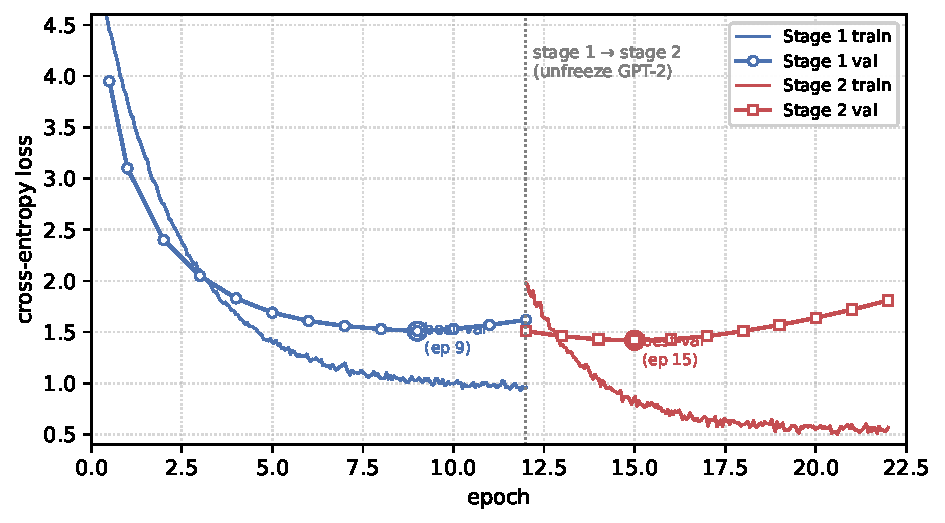
\includegraphics[width=\linewidth]{fig_loss.pdf}
\caption{Train and val cross-entropy across stages. Stage~1 (blue, 12
epochs, cross-attention only) overfits mildly: val loss is U-shaped with a
minimum around epoch~9. Stage~2 (red, 10 additional epochs, GPT-2 unfrozen)
overfits faster -- val loss reaches its minimum at epoch~15 and rises
sharply after. Both stages select the best-val checkpoint via
\texttt{load\_best\_model\_at\_end}.}
\label{fig:loss}
\end{figure}

\subsection{Future work}
Three directions look promising. First, \textbf{cross-domain evaluation}:
the original RECAP paper's strongest claim is that retrieval helps under
domain shift; testing AudioCaps$\rightarrow$Clotho with our pipeline is
mechanically straightforward and we see no reason it would not work given
more compute. Second, \textbf{larger/curated datastores}: \cite{ghosh2024recap}
augments the datastore with $600$k synthetic audio captions; replicating that
study and ablating composition (training-set-only vs.\ augmented) would
isolate retrieval quality from model capacity. Third, \textbf{audio-aware
re-ranking}: top-$k$ over CLAP cosine treats every retrieved caption equally;
a learned re-ranker that conditions on both the audio and the candidate
caption (e.g.\ a small bi-encoder) might recover the events that CLAP misses.

\section{Work Division}

\begin{table*}[t]
\begin{center}
\begin{tabular}{|l|c|p{8.5cm}|}
\hline
Student Name & Contributed Aspects & Details \\
\hline\hline
Mallika Lakshminarayan & \emph{[placeholder]} & \emph{[placeholder]} \\
Andrew J.\ Park        & \emph{[placeholder]} & \emph{[placeholder]} \\
Malhar Jadhav          & \emph{[placeholder]} & \emph{[placeholder]} \\
Harsh Gupta            & \emph{[placeholder]} & \emph{[placeholder]} \\
\hline
\end{tabular}
\end{center}
\caption{Contributions of team members. \emph{To be filled in.}}
\label{tab:contributions}
\end{table*}

The contributions of each team member are summarised in
Table~\ref{tab:contributions}. \emph{Detailed per-member descriptions to be
added.}

%-------------------------------------------------------------------------

{\small
\bibliographystyle{ieee_fullname}
\bibliography{egbib}
}

\end{document}
